\documentclass[11pt, letterpaper]{article}
\usepackage{amsmath, amssymb}
\usepackage{hyperref}
\usepackage{booktabs}
\usepackage{enumitem}
\usepackage{xcolor}
\usepackage{geometry}
\usepackage{fancyhdr}
\usepackage{titlesec}
\usepackage{tcolorbox}
\usepackage{graphicx}
\usepackage{caption}
\usepackage{subcaption}
\usepackage{parskip}
\geometry{margin=1in}

\definecolor{courseblue}{HTML}{002452}
\definecolor{coursegold}{HTML}{FABD0F}
\definecolor{coursered}{HTML}{B90E31}
\definecolor{lightblue}{HTML}{E8EEF7}
\definecolor{lightgold}{HTML}{FEF8E3}

\hypersetup{colorlinks=true,linkcolor=courseblue,urlcolor=coursered}
\tcbuselibrary{skins}
\newtcolorbox{guidancebox}{enhanced,colback=lightblue,colframe=courseblue,
  sharp corners,leftrule=4pt,left=6pt,right=6pt,top=4pt,bottom=4pt}

\pagestyle{fancy}\fancyhf{}
\fancyhead[L]{\small\textcolor{courseblue}{\textbf{CISC 473 --- Deep Learning | Fall 2026}}}
\fancyhead[R]{\small\textcolor{courseblue}{Final Report}}
\fancyfoot[C]{\small\thepage}
\renewcommand{\headrulewidth}{0.4pt}
\titleformat{\section}{\large\bfseries\color{courseblue}}{}{0em}{}[\titlerule]
\titleformat{\subsection}{\normalsize\bfseries\color{courseblue}}{}{0em}{}

\begin{document}
% Team review: confirm the contribution percentages and AI disclosure before submission.
{\centering
  {\Large\textbf{CISC 473: Deep Learning --- Final Report}}\\[0.6em]
  {\LARGE\bfseries Speaker-Independent Speech Emotion Recognition}\\[0.35em]
  {\large P20 --- Self-Supervised Features and Speaker Pitch Normalization}\\[0.65em]
  Nicholas Saloufakos, Connor Zakary, and Kaan Sun\\[0.35em]
  \href{https://github.com/nsaloufakos/Speech-Emotion-Recognition}{Project repository}
  \quad November 2026\\[0.45em]
  \rule{\linewidth}{0.4pt}\par
}

\begin{abstract}
Speech emotion recognition must generalize to unfamiliar speakers while retaining prosodic cues that help distinguish emotions. We compare three representations on the speech portion of RAVDESS under leave-one-speaker-out evaluation: mel-frequency cepstral coefficients with a bidirectional LSTM, frozen wav2vec~2.0, and frozen HuBERT. We investigate whether reducing between-speaker differences in pitch height improves recognition. Our waveform preprocessing estimates one robust pitch centre per speaker using active, high-strength frames from Praat filtered autocorrelation, then applies a constant pitch-synchronous shift toward 200 Hz. A bounded version limits the shift to four semitones in either direction. On a matched set of 1,429 recordings and three seeds, bounded normalization increased unweighted average recall by 0.65, 0.46, and 0.44 percentage points for the MFCC, wav2vec~2.0, and HuBERT systems, respectively. The corresponding paired speaker-resampling intervals included zero. Full shifts aligned measured pitch centres more closely, while bounded shifts had the highest observed mean recall for each model. In separate original-audio experiments, a validation-selected HuBERT layer probe reached 68.45\% recall on the full speech cohort, and a one-epoch, one-seed backbone fine-tuning run reached 53.06\% on the matched cohort. The results document a reproducible trade-off between pitch alignment and recognition and delimit the evidence for modest gains under unlabeled batch speaker calibration.
\end{abstract}

\section{Introduction}
Two speakers can express the same emotion with substantially different habitual pitch. At the same time, a speaker may use a change in pitch to convey emotion. Speaker normalization therefore needs to account for what signal it removes, at which level it operates, and what is available for an unseen speaker at inference. A method that re-centres every recording independently can reduce pitch differences between emotions expressed by the same speaker.

We ask whether a constant speaker-level pitch shift provides a useful input transformation for eight-class emotion recognition on held-out RAVDESS actors. Our contribution is an audited waveform procedure that combines a robust log-pitch centre, bounded pitch-synchronous synthesis, and a matched evaluation across three model families. We also identify where in HuBERT emotion is most readily decoded under linear probing and report a separate resource-limited backbone fine-tuning run.

\clearpage
\section{Related Work}
\textbf{Self-supervised speech representations.}
wav2vec~2.0 learns contextual representations through contrastive prediction over quantized targets, while HuBERT predicts cluster-derived targets in masked regions \cite{wav2vec,hubert}. SUPERB uses lightweight downstream heads to measure transfer to tasks such as emotion recognition. Its HuBERT Large entry reported 67.62\% accuracy on a four-class IEMOCAP task \cite{superb}. Our eight-class RAVDESS LOSO setting uses different data, labels, and model sizes, so that number provides context for transfer learning.

\textbf{Emotion cues across layers and time.}
Pepino et al.\ used learned mixtures of wav2vec~2.0 layers and reported 84.3\% average recall with speaker feature normalization in a seven-class, fixed-split RAVDESS setup \cite{pepino}. Their label mapping, actor split, and classifier differ from ours. SpeechFormer models multiple temporal scales with a hierarchical architecture \cite{speechformer}. We isolate depth by attaching an independent linear probe to the mean-pooled representation of each HuBERT layer, holding the probe design fixed.

\textbf{Speaker and pitch normalization.}
Gat et al.\ use an adversarial objective to suppress speaker information in the learned feature representation \cite{gat}. Our intervention operates directly on audio and can be reused across handcrafted and pretrained representations without a speaker-ID loss. Earlier experiments in our project used pYIN \cite{pyin}. The later audit compared low-energy and high-pitch estimates across detection methods, motivating active-frame selection and a robust centre rather than averaging all detected pitches.

\section{Method}
\subsection{Problem Formulation}
Given a mono utterance $x$ and one of eight emotion labels $y$, predict $y$ for a speaker excluded from supervised training. The normalized conditions additionally use unlabeled utterances from the test speaker to estimate their pitch centre. This models batch calibration. The original condition uses the utterance directly.

\subsection{Model Architecture}
\begin{center}
\small
\begin{tabular}{@{}ll@{}}
\toprule
Representation & Path to eight class logits \\
\midrule
40 MFCCs per frame & Packed BiLSTM (64 units/direction) $\to$ linear head \\
Frozen HuBERT or wav2vec~2.0 & Transformer states $\to$ temporal mean $\to$ linear head \\
Fine-tuned HuBERT & Trainable backbone $\to$ temporal mean $\to$ linear head \\
\bottomrule
\end{tabular}
\end{center}
For the BiLSTM, we concatenate the final forward and backward hidden states. For each frozen encoder, a 768-dimensional mean-pooled representation feeds a linear head. The main benchmark uses the final Transformer layer. The probes repeat the head training for layers 1--12 separately.

\subsection{Training Objective}
For logits $z$ and label $y$, the cross-entropy loss is
$\mathcal L=-\log\bigl(\exp(z_y)/\sum_{k=1}^{8}\exp(z_k)\bigr)$.
We select the epoch with the highest validation UAR and evaluate that checkpoint on the held-out actor.

\clearpage
\subsection{Proposed Modification}
Let $\mathcal A_{s,u}$ be the frames retained for utterance $u$ from speaker $s$. Praat 7.0.03 supplies filtered-autocorrelation pitch estimates on a 10 ms grid, within 50--800 Hz. We retain finite voiced estimates with candidate strength at least 0.6 and frame RMS within 35 dB of the utterance's maximum. We summarize each utterance in the log-frequency domain, then give each utterance equal weight when fitting the speaker centre:
\[
  b_s=\operatorname{median}_{u}
       \left(\operatorname{median}_{t\in\mathcal A_{s,u}}\log_2 F_{0,s,u}(t)\right),
  \qquad \Delta_s=12(\log_2 200-b_s).
\]
We apply $\Delta_s$ in the full condition and $\operatorname{clip}(\Delta_s,-4,4)$ in the capped condition. Each utterance from a speaker receives the same shift. An ideal constant semitone shift adds an offset to log pitch, preserving log-pitch differences within and between that speaker's utterances. The delivered waveform can depart from this ideal due to pitch tracking and synthesis.

We use pitch-synchronous overlap-add (PSOLA) through Parselmouth 0.4.7 with embedded Praat 6.1.38 at the source sampling rate. We then resample to 16 kHz and save floating-point WAVs. The current Praat executable measures pitch for the baseline and acoustic audit. The embedded version performs synthesis. Both conditions generated all 1,440 recordings.

\section{Experiments}
\subsection{Experimental Setup}
\textbf{Data and splits.} RAVDESS contains acted audiovisual speech and song \cite{ravdess}. We use the 1,440 speech-audio recordings from 24 actors, with neutral, calm, happy, sad, angry, fearful, disgust, and surprised labels. Every LOSO fold trains on 21 actors, validates on two, and tests on one. For all nine model-by-audio cells we use the same 1,429-recording intersection of original and historical variants. Keeping that cohort fixed prevents differences in included utterances from shifting the comparison. Original-layer probes use the full 1,440 recordings.

\textbf{Optimization and software.} Python, PyTorch, Hugging Face Transformers, librosa, and SoundFile implement loading, features, and training. We use the \texttt{facebook/hubert-base-ls960} and \texttt{facebook/wav2vec2-base} checkpoints. MFCC and frozen-head models use Adam, learning rate $10^{-3}$, batch size 32, and 30 epochs. Frozen-encoder experiments use the saved Mac runs and train heads on CPU. MFCC uses the packed BiLSTM on the RTX 3060. Within each model the execution setup is fixed across audio conditions. In the separate RTX HuBERT fine-tuning run, the backbone and head are both trainable, using Adam at $10^{-5}$, batch size 1, gradient checkpointing, and one epoch on original audio. That run uses seed 42 for all 24 folds.

\textbf{Metrics and checks.} Weighted average recall (WAR) is accuracy. UAR is the arithmetic mean of the eight class recalls. We pool held-out predictions across the 24 folds for each seed. The matched matrix reports mean and sample standard deviation across seeds 42, 123, and 999. Saved predictions were checked for correct test membership and independently rescored. We report the single-seed fine-tuning run without a seed standard deviation.

\clearpage
\subsection{Main Results}
\begin{table}[h!]
\centering
\caption{Matched test results (\%). Mean $\pm$ sample standard deviation over three seeds.}
\label{tab:main}
\begin{tabular}{@{}llrr@{}}
\toprule
Model & Audio & UAR & WAR \\
\midrule
MFCC--BiLSTM & Original & $35.65\pm2.18$ & $37.79\pm2.07$ \\
 & Full & $36.02\pm0.53$ & $38.35\pm0.50$ \\
 & Capped & $\mathbf{36.31}\pm2.87$ & $\mathbf{38.63}\pm3.00$ \\
wav2vec~2.0 & Original & $43.62\pm0.37$ & $44.65\pm0.39$ \\
 & Full & $44.05\pm1.06$ & $44.90\pm0.99$ \\
 & Capped & $\mathbf{44.09}\pm0.38$ & $\mathbf{45.18}\pm0.32$ \\
HuBERT & Original & $58.63\pm0.79$ & $59.60\pm0.51$ \\
 & Full & $58.54\pm0.62$ & $59.32\pm0.39$ \\
 & Capped & $\mathbf{59.06}\pm0.62$ & $\mathbf{59.79}\pm0.63$ \\
\bottomrule
\end{tabular}
\end{table}

Frozen HuBERT has the highest mean UAR among the matched final-layer and MFCC baselines for all three conditions. Capped normalization has the highest observed mean UAR within each model. Using unrounded scores, capped-minus-original differences are $+0.65$, $+0.46$, and $+0.44$ percentage points for MFCC, wav2vec~2.0, and HuBERT. The corresponding WAR differences are $+0.84$, $+0.53$, and $+0.19$ points. Paired 95\% speaker-resampling intervals for UAR are $[-1.30,2.68]$, $[-1.47,2.55]$, and $[-1.54,2.28]$ points. These are conditional estimates from 10,000 paired draws over held-out actors using fixed seed predictions. Each includes zero.

\textbf{HuBERT layer probing.} On the full original-audio cohort, layer 7 had the highest mean validation UAR (71.34\%). It reached $68.45\pm0.48$\% test UAR and $69.10\pm0.43$\% WAR. Layer 6 reached the highest observed test UAR ($69.38\pm0.31$\%), and layer 12 reached $59.92\pm0.95$\%. Layer 7 is the validation-selected result. The layer 6 maximum is descriptive, and these full-cohort results are reported separately from Table~\ref{tab:main}.

\textbf{HuBERT backbone fine-tuning.} The one-epoch experiment completed all 24 folds and produced 1,429 held-out predictions. It achieved 53.06\% UAR and 55.21\% WAR. On the same cohort and seed, frozen HuBERT achieved 59.54\% and 60.18\%, respectively. The fine-tuning result is 6.48 UAR points lower under its shorter training schedule. Follow-up runs with more epochs and seeds are needed to evaluate the effect of full adaptation.

\clearpage
\subsection{Ablation Study}
The full and capped conditions use the same estimator, target, and synthesis implementation, so this comparison tests how limiting shift magnitude affects recognition. Fourteen of 24 actors had requested full shifts beyond four semitones. Measured speaker centres spanned 98.89--294.05 Hz on original audio, 196.51--207.68 Hz after full alignment, and 125.05--237.74 Hz after capping. The median absolute discrepancy between the requested and measured recording-level median shift was about 0.019 semitones in both conditions. The stronger acoustic alignment did not translate into a better mean recognition score in these experiments.

In the earlier HuBERT comparison, per-utterance Librosa normalization reached 42.81\% UAR, utterance-level PSOLA reached 55.85\%, and capped speaker normalization with the previous pYIN mean reached 56.95\%. Replacing that baseline procedure with active-frame Praat medians at the same cap and with the same PSOLA implementation increased mean UAR by 2.12 points. The detector, frame selection, and summary statistic changed together. Isolating each factor would require fixing the other two.

\subsection{Qualitative Analysis}
In seed 42, the MFCC classifier changed actor 24's neutral recording
\texttt{03-01-01-01-02-01-24} from \emph{sad} on original audio to the correct
\emph{neutral} label after capping. For actor 7's calm recording
\texttt{03-01-02-01-01-01-07}, the same transformation changed a correct prediction to \emph{sad}. These paired examples show both directions of change on the same speaker-disjoint protocol. An individual flip cannot identify which acoustic cue the model relied on.

\subsection{Failure Analysis}
\textbf{Pitch-estimator instability.} For the audited actor 3 happy recording
\texttt{03-01-03-01-01-01-03}, legacy pYIN estimates moved from about 175 Hz to 273 Hz across the original and utterance-normalized recordings. On the 35 frames voiced in both, the corresponding means were closer to 176 Hz and 205 Hz. Comparing matched voiced frames and filtering quiet estimates makes these diagnostics less sensitive to changing frame sets.

\textbf{Large shifts and local deviations.} Full normalization requested shifts as large as $+12.19$ semitones. About 5\% of shared strong frames differed from the requested shift by more than one semitone. Timing differences, detector ambiguity, and synthesis can all contribute. Capping avoids the largest requested shifts. A zero-shift PSOLA control, which was not run, could help quantify the effects of resynthesis alone.

\textbf{Uneven class recall after short fine-tuning.} The one-epoch HuBERT model recalled 89.58\% of calm examples and 16.32\% of sad examples. Pooled UAR exposes this disparity even when accuracy appears higher. A follow-up should compare longer training schedules and inspect actor-level confusions to test whether the disparity is stable.

\clearpage
\section{Discussion}
The main contribution is a reusable input intervention whose acoustic behavior and downstream performance can be checked separately. The paired results suggest that bounded shifts are a better candidate than exact alignment on this corpus. The largest repeatable descriptive recovery is relative to the earlier normalization pipeline, while improvements over original audio remain modest.

\subsection{Limitations}
RAVDESS contains acted performances and a small set of scripted statements. Generalization to spontaneous speech, new languages, and other microphones remains open. Normalized inference assumes a batch of unlabeled recordings from each test speaker. Its effectiveness with a small, separate calibration set or a first utterance remains unknown. The speaker intervals condition on trained models and fixed seeds and do not account for the overlap of LOSO training sets. Additional proposal experiments such as normalized-layer probing, wav2vec~2.0 backbone fine-tuning, and training-only augmentation were outside the completed comparison.

\section{Conclusion}
Frozen HuBERT performed best in the nine-cell matched comparison. Capped speaker normalization produced small positive mean UAR differences across all three model families, with speaker-resampling intervals spanning zero. Measuring pitch before and after synthesis revealed a useful distinction between aligning a speaker statistic and improving emotion classification. Future evaluation should test a separate calibration batch, include a resynthesis control, and repeat fine-tuning across training schedules.

\section{AI Tool Disclosure}
ChatGPT/Codex assisted with code drafting and debugging, environment setup and execution, result verification and interpretation, and preparation of this report draft. The team should review this disclosure and confirm that it reflects the actual use of AI tools across members before submitting.

\section{Contribution Declaration}
The proposal lists the roles below. Each member should add their actual completed contributions and agree on percentages that total 100\%.
\begin{center}
\small
\begin{tabular}{@{}lll@{}}
\toprule
Member & Proposal role & Final contribution \\
\midrule
Nicholas Saloufakos & Project lead & \textit{Team to confirm tasks and share} \\
Connor Zakary & Research lead & \textit{Team to confirm tasks and share} \\
Kaan Sun & Engineering lead & \textit{Team to confirm tasks and share} \\
\bottomrule
\end{tabular}
\end{center}

\clearpage
\renewcommand{\refname}{References}
\begin{thebibliography}{9}\small
\bibitem{ravdess} S. R. Livingstone and F. A. Russo.
The Ryerson Audio-Visual Database of Emotional Speech and Song.
\textit{PLOS ONE}, 2018. \href{https://doi.org/10.1371/journal.pone.0196391}{DOI}.
\bibitem{wav2vec} A. Baevski et al.
wav2vec 2.0: A Framework for Self-Supervised Learning of Speech Representations.
\textit{NeurIPS}, 2020. \href{https://arxiv.org/abs/2006.11477}{Paper}.
\bibitem{hubert} W.-N. Hsu et al.
HuBERT: Self-Supervised Speech Representation Learning by Masked Prediction of Hidden Units.
\textit{IEEE/ACM TASLP}, 2021. \href{https://arxiv.org/abs/2106.07447}{Paper}.
\bibitem{superb} S.-W. Yang et al. SUPERB: Speech Processing Universal PERformance Benchmark.
\textit{Interspeech}, 2021. \href{https://arxiv.org/abs/2105.01051}{Paper}.
\bibitem{pepino} L. Pepino, P. Riera, and L. Ferrer. Emotion Recognition from Speech Using wav2vec 2.0 Embeddings.
\textit{Interspeech}, 2021. \href{https://www.isca-archive.org/interspeech_2021/pepino21_interspeech.pdf}{Paper}.
\bibitem{speechformer} W. Chen et al. SpeechFormer: A Hierarchical Efficient Framework Incorporating the Characteristics of Speech.
\textit{Interspeech}, 2022. \href{https://arxiv.org/abs/2203.03812}{Paper}.
\bibitem{gat} I. Gat et al. Speaker Normalization for Self-Supervised Speech Emotion Recognition.
\textit{ICASSP}, 2022. \href{https://arxiv.org/abs/2202.01252}{Paper}.
\bibitem{pyin} M. Mauch and S. Dixon. pYIN: A Fundamental Frequency Estimator Using Probabilistic Threshold Distributions.
\textit{ICASSP}, 2014. \href{https://doi.org/10.1109/ICASSP.2014.6853678}{DOI}.
\end{thebibliography}

\clearpage
\appendix
\section{Additional Results}
\begin{figure}[h!]
\centering
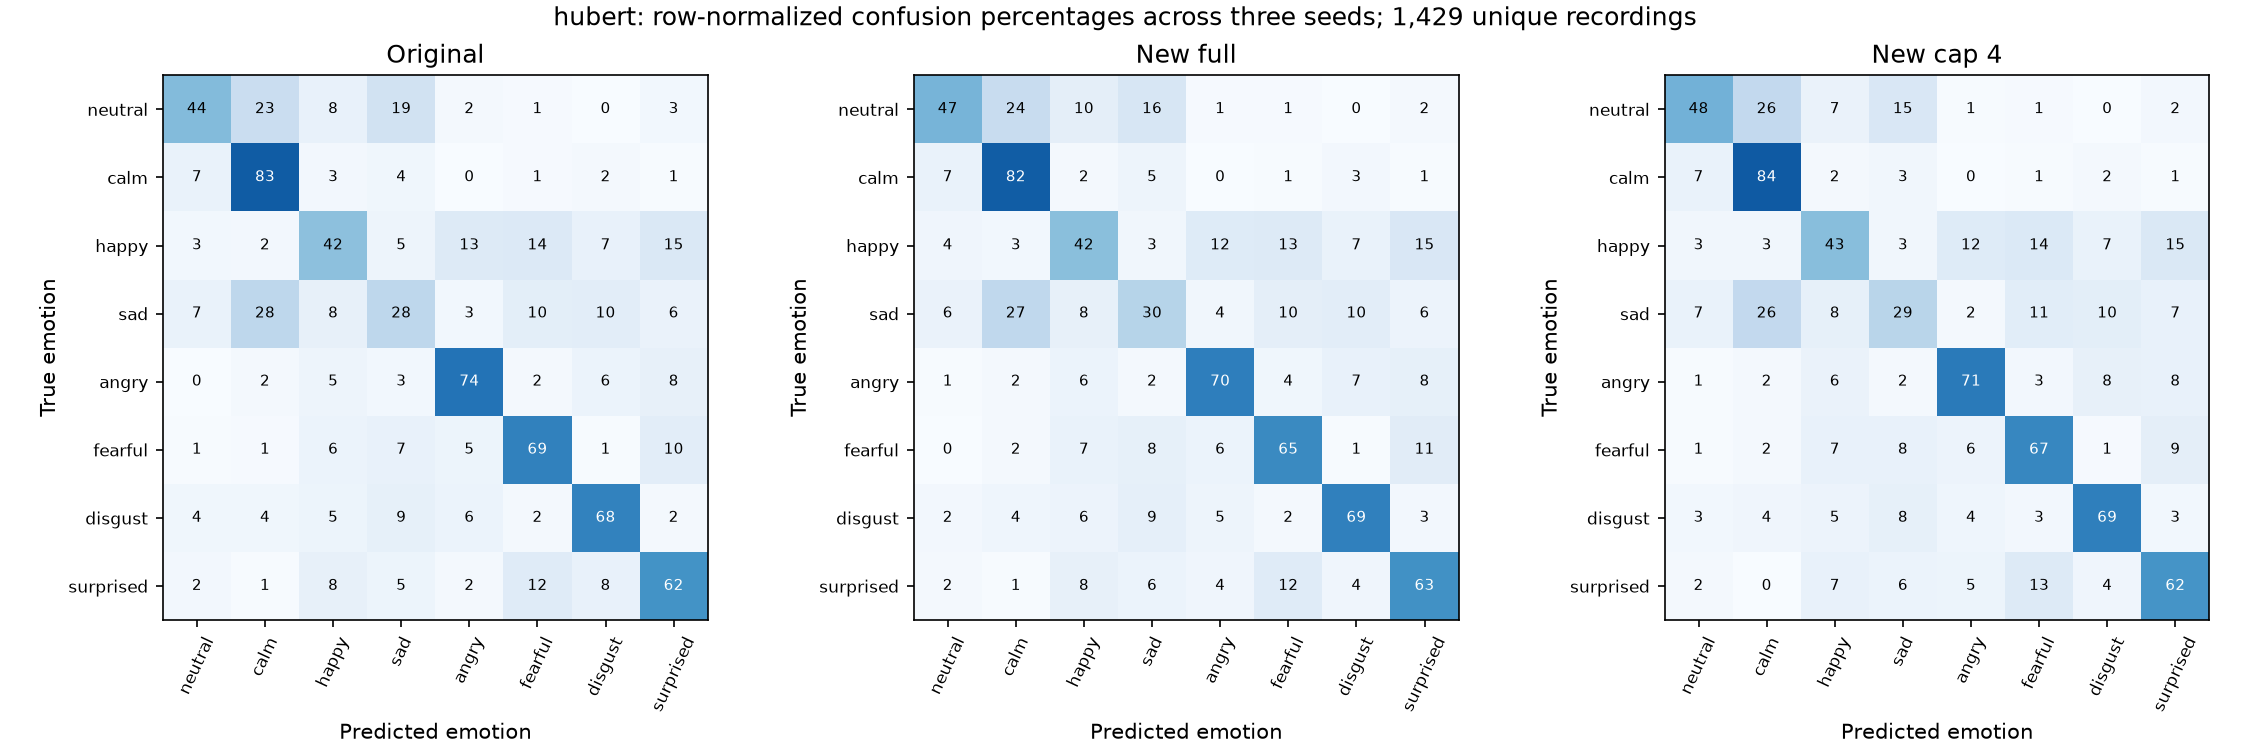
\includegraphics[width=\linewidth]{../analysis/model_comparison_cuda/hubert_confusions.png}
\caption{Frozen HuBERT row-normalized confusion matrices across audio conditions. Each panel pools predictions from the same held-out cohort over three seeds.}
\end{figure}

\textbf{Per-emotion recall for one-epoch HuBERT.} Neutral 19.79\%, calm 89.58\%, happy 24.48\%, sad 16.32\%, angry 70.68\%, fearful 55.73\%, disgust 77.66\%, and surprised 70.21\%.

\section{Reproducibility Checklist}
\begin{itemize}[nosep]
\item Use \texttt{README.md} for environment setup, checkpoint caching, audio restoration, and evaluation commands.
\item Preserve \texttt{output/splits.csv} and the matched cohort CSV in \path{output/pitch_comparison_hubert/}. Report metrics after pooling held-out predictions within each seed.
\item Run the matched MFCC evaluator with original, capped, and full conditions and pass the regenerated waveform root through \texttt{--variant-root}. Historical frozen results and the verified combined summary are retained in the repository.
\item For the original-audio fine-tuning run, use the cached HuBERT checkpoint and run \path{src/evaluate_hubert_finetuned.py} with \texttt{--seeds 42 --epochs 1} and a new \texttt{--output-root}. The runner defaults to all 24 folds.
\item The pitch audit, normalization diagnostics, and generation summaries are under \path{analysis/pitch_validation/}. Evaluation artifacts retain predictions and configuration details for independent rescoring.
\end{itemize}
\end{document}
